\documentclass{standalone}
\usepackage{tikz}

\begin{document}
	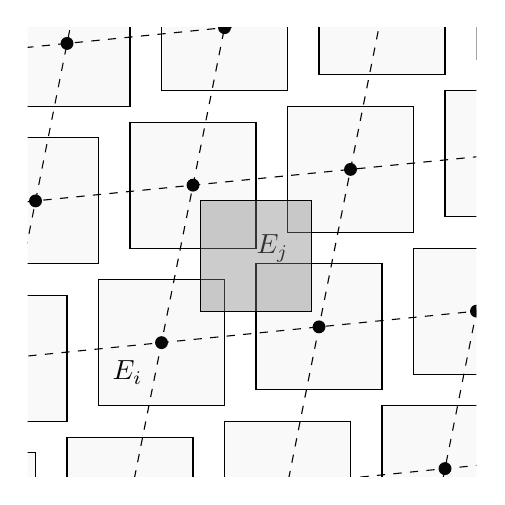
\begin{tikzpicture}
	%copied from www.texample.net/tikz/examples/lattice-points/ and suitably modified
	
	
	\clip (-1.7,-1.7) rectangle (4cm,4cm); % Clips the picture...
	
	\def\l{2};
	\def\s{0.4};
	\def\S{0.35};
	
	\def\A{1}
	\def\B{0.1}
	\def\C{0.2}
	\def\D{1}
	\begin{scope}
	\pgftransformcm{\A}{\B}{\C}{\D}{\pgfpoint{0cm}{0cm}}
	% This is actually the transformation matrix entries that
	% gives the slanted unit vectors.

	\draw[dashed] (-4,-4) grid[step=\l cm] (7,7);
	% Draws a grid in the new coordinates.
	
	\foreach \x in {-4,-3,...,3}{% Two indices running over each
		\foreach \y in {-4,-3,...,3}{% node on the grid we have drawn 
			\node[draw,circle,inner sep=1.5pt,fill] at (\l*\x,\l*\y) {};
			% Places a dot at those points
		}
	}
	
	\node at (-0.1,-0.1) [below left] {$E_i$};
	
	\node at (0.5*\l-0.08,0.5*\l-0.19) [above right] {$E_j$};
	
	
	%\node at (0.5*\l,0.5*\l) {$D$};
	\end{scope}
	
	
	\foreach \x in {-1,-2,0,1,2}{% Two indices running over each
		\foreach \y in {-1,-2,0,1,2}{% node on the grid we have drawn 
			\filldraw[fill=gray, fill opacity=0.05, draw=black] (-\s*\l+\x*\l*\A+\y*\l*\C,-\s*\l+\x*\l*\B+\y*\l*\D)
			rectangle (\s*\l+\x*\l*\A+\y*\l*\C,\s*\l+\x*\l*\B+\y*\l*\D);
			
		}
	}
	
	\filldraw[fill=gray, fill opacity=0.4, draw=black] ({-\S*\l+0.5*\l*(\A+\C)},{-\S*\l+0.5*\l*(\B+\D)})
	rectangle ({\S*\l+0.5*\l*(\A+\C)},{\S*\l+0.5*\l*(\B+\D)});
	
	\end{tikzpicture}
\end{document}